\section{Experimental Setup}
\label{sec:setup}

In this section, we describe how the data were generated and evaluated. Section~\ref{subsec:channel-simulation} describes the channel simulation; Sections~\ref{subsec:studies}--\ref{subsec:device-model} describe the deployments, the mobility and the devices, and Sections~\ref{subsec:features}--\ref{subsec:protocol} the features, estimators and evaluation protocol.

\subsection{Channel Simulation}
\label{subsec:channel-simulation}

% src: FINAL_REPORT.md §4.2; configs (*_15x15, *_25x25: bandwidth 1e8)
All data are generated with QuaDRiGa, a 3GPP TR~38.901-compliant channel simulator~\cite{3gpp38901,quadriga_paper,quadriga_website}, at \SI{3.0}{\giga\hertz} center frequency with \SI{100}{\mega\hertz} bandwidth, with $256$ orthogonal frequency-division multiplexing~(OFDM) subcarriers, \SI{30}{\dBm} transmit power per site, and an omnidirectional BS antenna element. This work extends a time-aware multi-user massive multiple-input multiple-output~(MIMO) simulator developed within the same research group~\cite{Israeli_5G_Massive_MIMO_2026,israeli_sarne_simulation}, to which we added grid-constrained trajectory generation and the device-heterogeneity model that is described in Section~\ref{subsec:device-model}.

% src: FINAL_REPORT.md §4.2 ("What interference means here")
Where a deployment includes interfering BSs in addition to the serving BS, SINR is computed as
\begin{equation}
  \mathrm{SINR} = \frac{P_{\text{serving}}}{\sum_i P_{\text{IBS-}i} + P_{\text{noise}}},
  \label{eq:sinr}
\end{equation}
where $P_{\text{serving}}$ and $P_{\text{IBS-}i}$ are the received powers from the serving BS and the $i$-th interfering BS, and $P_{\text{noise}} = \SI{-104}{\dBm}$ is the noise power, a fixed setting of the simulation. Interference is therefore contributed only by the modeled interfering sites; no user-to-user coupling is represented, and a user's SINR does not depend on how many other users are simulated.

\subsection{Studies}
\label{subsec:studies}

% src: FINAL_REPORT.md §4.1, §7.5 ("eight differences"); technical_documentation.md §3, §7.1, §7.3.3, §7.4; configs/multi_user_voronoi_15x15_config.jsonc, ne_bs_voronoi_15x15_config.jsonc, ne_bs_voronoi_25x25_config.jsonc (center_frequency, grid, base_station)
We draw the evidence from three simulated deployments at two scales, summarized in Table~\ref{tab:studies}. The \emph{controlled-grid study} places UEs on a $15\times15$ grid at \SI{2}{\meter} pitch within \SI{20}{\meter} of the serving BS and predicts the exact cell, under conditions chosen to be clean and repeatable. The \emph{macro-cell study} places $300$ users on a $25\times25$ grid at \SI{4}{\meter} pitch, $21$ to \SI{157}{\meter} from an off-grid serving BS, predicts continuous position, and evaluates on users never seen during training. The \emph{$25\times25$ regression runs} share the macro-cell geometry but, like the controlled grid, split each user's walk in time; they simulate five device profiles, one user each, pooled in one model, under three propagation settings: urban-micro~(UMi) line-of-sight~(LOS), uniform UMi non-line-of-sight~(NLOS), and a per-cell mix of the two. As a design choice, the reference history depth is $h=3$ in the controlled-grid study and the $25\times25$ runs and $h=5$ in the macro-cell study; the sequence models of the first two are evaluated up to $h=15$, and other depths are stated where used. A fourth deployment, a corridor with a blocked line of sight, is described in Section~\ref{subsec:robustness}.

\begin{table}[t]
  \centering
  \caption{The three simulated deployments.}
  \label{tab:studies}
  \small
  \begin{tabularx}{\textwidth}{@{}lXXX@{}}
    \toprule
     & Controlled-grid study & $25\times25$ regression runs & Macro-cell study \\
    \midrule
    Task & Classification~(225 cells) & Regression & Regression \\
    Grid, pitch & $15\times15$, \SI{2}{\meter} & $25\times25$, \SI{4}{\meter} & $25\times25$, \SI{4}{\meter} \\
    Service area & \qtyproduct{28 x 28}{\meter} & \qtyproduct{96 x 96}{\meter} & \qtyproduct{96 x 96}{\meter} \\
    Range to serving BS & $0$--\SI{20}{\meter}~(center BS); $21$--\SI{61}{\meter}~(corner BS) & $21$--\SI{157}{\meter} & $21$--\SI{157}{\meter}, mean \SI{93}{\meter} \\
    Serving BS~(m) & $[19,19,10]$~(center) or $[48,48,10]$~(corner) & $[116,116,10]$ & $[116,116,10]$ \\
    Carrier & \SI{3.0}{\giga\hertz} & \SI{3.0}{\giga\hertz} & \SI{3.0}{\giga\hertz} \\
    Population & 5 device profiles, $450{,}005$ samples & 5 device profiles, one user each, $1{,}250{,}000$ samples, \SI{30}{\percent} of training samples used & 300 users simulated, 232 retained, 47 tested per split \\
    Split & Chronological $80/20$ within each user & Chronological, or shuffled 5-step blocks & $80/20$ over disjoint users \\
    Mobility & Random walk, \SI{1.5}{\meter\per\second} & Random walk & Four patterns, $0.1$--\SI{15}{\meter\per\second} \\
    AoA impairment & SINR-dependent noise, \ang{5} quantization & \ang{4} Gaussian noise, \ang{5} quantization & \ang{4} Gaussian noise, \ang{5} quantization \\
    Repetitions & Single run~(trees); three seeds~(sequence models) & Single run; three seeds for the GRU at $h=15$ & $20$ user splits~(XGBoost, Random Forest); five~(other models) \\
    \bottomrule
  \end{tabularx}
\end{table}
% src (macro-cell AoA impairment): CSI-Location src/python/utils/csi_dataset.py load_and_prepare_data (aoa_noise_std_deg=4.0, aoa_quant_step_deg=5.0); 232 retained: FINAL_REPORT.md §4.3; 47 test users: seed_repeats_all_models_summary.json per-run n_test_users; range 21.2-157.0 m, mean 93.2: FINAL_REPORT.md §7.5

% src: configs/multi_user_voronoi_15x15_config.jsonc (BS [19,19,10]; interferers [-11,19,10], [19,-11,10]); ne_bs_voronoi_15x15_config.jsonc (BS [48,48,10]; same interferers); both read by core/generate_simulation_data.m; technical_documentation.md §7.3 (~52 degree azimuth spread)
% src: results_of_record/controlled_grid_2026_10/comparison_sets.md (RMa LOS, mixed per-cell, uniform NLOS at 3.0 GHz)
In the controlled-grid study the serving BS sits either at the grid center, where the grid spans the full \ang{360} of azimuth, or beyond the north-east corner, where all $225$ cells fall within a wedge of about \ang{52}; two interfering sites enter through Equation~(\ref{eq:sinr}) for both placements. The grid is simulated under three propagation settings: rural-macro~(RMa) LOS for every walk; a mixed setting in which each of four Voronoi zones has its own UMi LOS or NLOS scenario, so that the propagation changes along a walk; and uniform UMi NLOS. Figure~\ref{fig:layout} draws the controlled grid and the macro cell to the same scale.

% src: configs/ne_bs_voronoi_25x25_config.jsonc (BS [116,116,10]); FINAL_REPORT.md §4.1 (interferers); FINAL_REPORT.md §5.6 (uniform NLOS primary); CONTINUE_HERE.md §3 (per-segment mixed runner)
In the macro-cell study the serving BS sits off-grid to the north-east, again with two interfering sites. The primary realization of this study uses a single UMi NLOS propagation profile for every user. A second realization assigns each of four Voronoi regions its own profile, LOS for the park to the north and the highway to the south-west and NLOS for the shopping district to the south-east and the residential area to the south, and generates each scenario segment of a trajectory as an independent channel; it serves to test how propagation conditions change the result.

\begin{figure}[h]
  \centering
  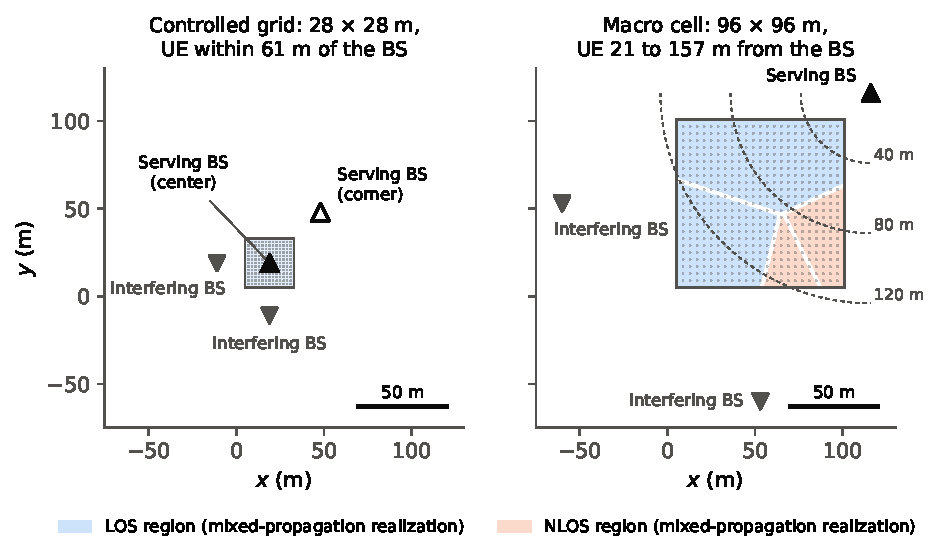
\includegraphics[width=0.95\textwidth]{fig_study_maps}
  \caption{The controlled grid with its two serving-BS placements~(left) and the macro cell with its four Voronoi regions~(right), at the same scale. Filled and open markers give the center and corner placements; arcs give the range from the macro-cell BS.}
  \label{fig:layout}
\end{figure}
% src: figure_scripts/python/make_figures.py study_maps(); grids, BS positions and Voronoi centres from the 15x15 and 25x25 configs; macro-cell transmitters from runners/run_multi_user_300_25x25.m (the 25x25 config's interferer entries, [-25,53] and [53,-25], are not used by that runner)


\subsection{Mobility}
\label{subsec:mobility}

% src: FINAL_REPORT.md §4.3
The controlled-grid study moves each UE on a random walk over the $8$-connected grid graph at \SI{1.5}{\meter\per\second}; the walk carries no persistent heading. In the macro-cell study each user follows one of four trajectory patterns, namely boundary-reflecting straight-line navigation, a persistent random walk, a waypoint tour or a straight transit, at a speed between \SI{0.1}{\meter\per\second}~(near-static) and \SI{15}{\meter\per\second}~(vehicular). All four patterns carry heading persistence, so the mobility of the macro cell favors the use of a history of reports.

% src: FINAL_REPORT.md §4.3, §5.8 (every step advances exactly one grid cell); jitter: generate_simulation_data.m l.238-241 (grid, 25x25 runs); none in run_multi_user_300_25x25*.m (macro)
In all three studies, every step of a walk advances exactly one grid cell, and the time between snapshots is the step length divided by the UE's speed. A fixed history depth is therefore a fixed distance travelled, $h$ grid steps, but not a fixed duration: across the $232$ retained macro-cell users the time between snapshots $\Delta t$ ranges from $0.27$ to \SI{32.5}{\second}, with a median of \SI{2.71}{\second}. In the controlled-grid study and the $25\times25$ runs, a jitter of \SI{+-0.1}{\meter} is added to every snapshot so that no estimator can latch onto repeated coordinates; in the macro-cell study, by contrast, the snapshots lie exactly on the grid points.

\subsection{Device Model and AoA Impairment}
\label{subsec:device-model}

% src: FINAL_REPORT.md §4.4; technical_documentation.md §3.6, §3.7
The controlled-grid study simulates five device profiles: two four-antenna devices that differ only in their walk, a two-antenna device, a one-antenna device, and a two-antenna device carried at \SI{0.9}{\meter} height. The macro-cell study draws from a population of \SI{85}{\percent} multi-antenna devices~(about \SI{45}{\percent} with four antennas and \SI{40}{\percent} with two) and \SI{15}{\percent} single-antenna devices, each with its own antenna gain and carrying height. The split is an assumption of this work.
Antenna count enters the channel through Equation~(\ref{eq:mrc}), and AoA capability is imposed when features are built.

% src (footnote): CLAIM_EVIDENCE_MAP.md C7 (single omni BS; AoA = simulator angle + noise, generate_simulation_data.m)
% src: FINAL_REPORT.md §4.4 (SINR-dependent model, controlled grid); csi_dataset.py load_and_prepare_data (macro cell: aoa_noise_std_deg = 4.0, aoa_quant_step_deg = 5.0, AoA = 0 for single-antenna devices)
Clean simulated arrival angles are degraded before use.\footnote{The serving BS has a single omnidirectional element, so the reported AoA is not estimated from an array response; it is the arrival angle of the simulated channel, degraded as described here.} In the controlled-grid study the noise on each axis depends on SINR,
\begin{equation}
  \sigma_{\text{AoA}}(t) = \operatorname{clamp}\!\left(2.0^\circ \cdot 10^{-\frac{\mathrm{SINR}_{dB}(t)-10}{15}},\ 1.0^\circ,\ 20.0^\circ\right),
  \label{eq:aoa-noise}
\end{equation}
whereas the macro-cell study and the $25\times25$ runs apply a fixed Gaussian error of standard deviation $\sigma_{\text{AoA}} = \ang{4}$, drawn independently for every report. Both then quantize azimuth and elevation to a codebook of step $\Delta_{\text{q}} = \ang{5}$. Both impairment models are fixed settings of the simulation pipeline, and Section~\ref{subsec:averaging} varies them. Single-antenna devices cannot form a beam and report no angle; in the macro-cell features their angle is set to \ang{0}.

\subsection{Features}
\label{subsec:features}

% src: technical_documentation.md §4.1-4.3
In the controlled-grid study, $\mathbf{m}(t)$ contains RSS and SINR, optionally extended with the AoA pair and with three device parameters: antenna count, antenna gain, and carrying height. The window of Equation~(\ref{eq:transition-history}) is built per user after sorting by time; the first $h$ snapshots of each user are dropped, and no window crosses from one user to another. Values are stacked in absolute form, because device-specific RSS and SINR offsets are stable and act as fingerprints.

% src: FINAL_REPORT.md §4.5; csi_dataset.py build_derived_features (d_rss, d_az, d_ray_x, d_ray_y are per-user first differences divided by delta_t; ray = FSPL range estimate x AoA unit vector)
In the macro-cell study, each snapshot carries $13$ channels, all computable from the raw measurements: RSS; SINR; the sines and cosines of both angles; two ray-projection coordinates formed from a path-loss range estimate and the AoA unit vector; the time increment $\Delta t$; and the first differences of RSS, azimuth and the two ray coordinates, each divided by $\Delta t$. It should be noted that, because the first differences are part of each snapshot, the $h=0$ input of the macro-cell study already contains one step of change, and the $h=5$ input stacks six such snapshots. Three static device features, namely antenna count, gain and height, accompany every input.

\subsection{Estimators}
\label{subsec:estimators}

% src: CSI-Location experiments_ablation/model_zoo.py (build_classical, build_net, training constants); master_benchmark_rerun_summary.json (n_params)
The macro-cell study evaluates seven estimators spanning five algorithmic paradigms, listed in Table~\ref{tab:estimators}: $k$-NN, Random Forest, XGBoost, a gated recurrent unit~(GRU) network, and three one-dimensional convolutional neural networks~(1D-CNN), one with an AoA-validity channel and one with temporal self-attention. We hold the hyperparameters fixed across history depths, so that the input window is the only factor that varies within a model; their values are given in Appendix~\ref{app:hyperparameters}. The controlled-grid study uses Random Forest and XGBoost classifiers together with a 1D-CNN and a GRU, and the $25\times25$ runs use Random Forest and XGBoost regressors together with the same two sequence models.

\begin{table}[h]
  \centering
  \caption{Estimators used in the macro-cell study.}
  \label{tab:estimators}
  \small
  \begin{tabular}{@{}lll@{}}
    \toprule
    Paradigm & Model & Configuration \\
    \midrule
    Instance-based & $k$-NN & $k=5$ \\
    Bagged trees & Random Forest & 150 trees, depth 16, min.\ leaf 5 \\
    Boosted trees & XGBoost & 50 trees, depth 5, learning rate 0.15 \\
    Recurrent & GRU & 2 layers, 254\,K parameters \\
    Convolutional & 1D-CNN & 3 convolutional layers, 67\,K parameters \\
    Convolutional & Mask-aware 1D-CNN & 1D-CNN with an AoA-validity channel, 67\,K parameters \\
    Attention & 1D-CNN with temporal self-attention & 200\,K parameters \\
    \bottomrule
  \end{tabular}
\end{table}

\subsection{Evaluation Protocol}
\label{subsec:protocol}

% src: FINAL_REPORT.md §4.7; technical_documentation_revised.md 6.2/6.4 (validation block from the training data for the grid and 25x25 sequence models)
The controlled-grid study and the $25\times25$ runs split each user's walk in time, training on the first \SI{80}{\percent} of steps and testing on the last \SI{20}{\percent}; a random split would leak, because spatial consistency makes temporally adjacent samples near-duplicates. The controlled grid is scored by exact-cell accuracy and by the mean distance between the predicted and true cells. The macro-cell study splits over users, so that the $47$ test users of each split are never seen during training, and it is scored by the 2D Euclidean error between predicted and true position. Every macro-cell result is reported separately for multi-antenna and single-antenna devices.

% src: seed_repeats_all_models.py docstring (seed drives split and init; marginal vs seed-paired); followup_2026_10 (20 seeds, XGBoost and RF, Student-t)
The primary comparison is the change in error when history is added, measured within one model against its own $h=0$ input. For the macro-cell results we repeat the whole protocol over $20$ seeds for XGBoost and Random Forest and over five for the other models, each seed drawing a different user split and model initialization. The spread across seeds is dominated by which users land in the test set; the seed-paired difference compares two inputs on the same split and thereby cancels that source, and its \SI{95}{\percent} Student-$t$ confidence interval is reported with each gain.

% src: experiments_ablation/model_zoo.py train_deep docstring (early stopping on test MAE)
The neural models of the macro-cell study select their stopping epoch by error on the test users, whereas those of the controlled grid and the $25\times25$ runs use a validation block taken from the training data. The macro-cell rule applies equally to both depths of a model, so within-model comparisons are unaffected; however, it makes the absolute errors of the neural models, and any comparison between them and the other models, optimistic in their favor.
